% Chapter 06 - Postop CRP and complications

\chapter{An investigation into the relationship between postoperative systemic inflammation and complications after pancreaticoduodenectomy.}
\label{ch_crp_comp}

\lhead{Chapter \ref{ch_crp_comp}. \emph{Postoperative CRP and complications}} % This is for the header on each page - perhaps a shortened title

\clearpage
%----------------------------------------------------------------------------------------
\section{Introduction}
Pancreaticoduodenectomy is associated with significant morbidity in spite of advances in patient selection, perioperative care and surgical technique. Early identification of complications can help improve outcomes by better allocation of critical care resources as well as goal-directed therapy. Postoperative pancreatic fistula is one of the most dreaded complications after a pancreaticoduodenectomy and can lead to a cascade of other complications including delayed haemorrhage, infected intra-abdominal collections, delayed gastric emptying, prolonged hospitalisation and in some cases, death. The International Study Group for Pancreatic Fistula (ISGPF) have not only defined what constitutes a post-operative pancreatic fistula but have also graded the severity of this complication based on its impact on the management of the patient. However, these definitions are applied after the event and there is no clear way of predicting the severity of complications.

Postoperative CRP levels have been shown to predict infective complications after major surgery including colorectal,  oesophago-gastric and pancreatic surgery. \parencite{mustard_c-reactive_1987, matthiessen_increase_2008, mcneer_early_2010, dutta_persistent_2011, mackay_c-reactive_2011, murakami_soft_2008, welsch_persisting_2008} It has been postulated that an unmitigated and exaggerated systemic inflammatory response in the early postoperative period is followed by a compensatory anti-inflammatory response that predisposes the patient to sepsis and impaired healing. 

But, the mechanisms underlying the pathogenesis of post-operative pancreatic fistula are largely attributed to anatomical factors including soft texture of the pancreas and small pancreatic duct diameter as well as surgical technique with increased intra-operative blood loss and pancreatico-jejunostomy rather than pancreatico-gastrostomy being associated with increased incidence of anastomotic leakage. The association between the early postoperative systemic inflammatory response and the incidence and severity of postoperative pancreatic fistula has not been reported. Moreover, the role postoperative CRP in predicting infective complications when these occur in association with postoperative pancreatic fistula has not been studied either. 

The aim of this study was to investigate the association between systemic inflammation, postoperative pancreatic fistula and infective complications in patients undergoing pancreaticoduodenectomy.

\section{Methods}
\todo{Check dates for this study}
Patients who underwent elective pancreaticoduodenectomy between January 2008 and July 2012 were included in this study. Patients who underwent only a trial dissection or trial dissection and surgical bypass during this period were excluded. All patients were given antibiotic prophylaxis at induction and this was continued for 24 hours after surgery. All patients had general anaesthesia supplemented either with patient-controlled epidural analgesia or spinal diamorphine and patient-controlled opiate analgesia for postoperative pain relief. Octreotide (200$\mu$g) was administered subcutaneously three times a day for 5 days in all patients and continued longer in patients diagnosed with a postoperative pancreatic fistula. Patients were routinely admitted to the surgical high dependency unit where a standardised regimen was followed for early mobilisation, chest physiotherapy and early enteral nutrition. All patients had one or two surgical drain(s) placed at the time of surgery which were removed at the clinician's discretion during the postoperative period based on the presence or absence of postoperative pancreatic fistula or other intra-abdominal collections. 

Patients had routine measurements of inflammatory markers including C-reactive protein (CRP) and differential white cell counts from the day before surgery and every day for at least a week after surgery. These results including the preoperative blood tests and the postoperative blood tests for the first 7 days after surgery were collected from the hospital laboratory databases.

All complications were discussed at a weekly morbidity meeting and prospectively recorded in an electronic database.  The diagnosis and grading of pancreas-specific complications including postoperative pancreatic fistula (POPF, Section \ref{sec:ch_intro_POPF}) and post-pancreatectomy haemorrhage (PPH, Section \ref{sec:ch_intro_PPH}) were made according to the International Study Group classifications as shown in Table \ref{table:isgps_popf} and Table \ref{table:isgps_pph} on p\pageref{table:isgps_popf} respectively.

All other complications were graded using the Clavien-Dindo classification system as shown in Table \ref{table:clavien-dindo}. This allowed the grading of the severity of the complications based on the magnitude of the intervention(s) required to treat them. Postoperative mortality was defined as death within 30-days of the operation or while still in hospital after the operation. Re-intervention in the form of radiological, endoscopic or surgical procedures was recorded prospectively.

\subsection{Statistics}
Mann-Whitney U test was used to compare the distribution of postoperative CRP (as a continuous variable) in patients who had a complication and those who did not. Data are presented as median (inter-quartile range, IQR) unless otherwise specified. Line plots with error bars depicting 95\% confidence intervals are used to depict the trends in CRP over time across different patient groups. 

Receiver operating characteristic (ROC) analysis \parencite{robertson_use_1981,zweig_receiver-operating_1993} was used to identify the optimum thresholds for postoperative CRP for predicting infective complications with a preference for thresholds that had a greater negative predictive value. Patients were categorised using these thresholds to analyse the relationship between CRP (as a categorical variable) and re-operation, hospital stay, critical care stay, number of critical care admissions as well as postoperative mortality using the Chi-square test. 

SPSS software (Version 22.0; IBM, USA) was used to perform statistical analysis. Effects were considered significant at $\alpha \leq0.05$. 

\todo{Complete this section - most of this can be modified from the stats sections in other chapters}


\section{Results}
\subsection{POPF, infective complications and other outcomes}
Pancreaticoduodenectomy was performed in 188 patients (126 male, 67\%) during the study period. The median age was 63.5 years (IQR 54 - 70 years). 79 (42\%) patients were over the age of 65 years. 

Post-operative pancreatic fistula (POPF) as defined by the International Study Group for Pancreatic Fistula (ISGPF) occurred in 62 (33\%) patients. Of these patients, 19 (10.1\%) had a Grade A POPF, 25 (13.3\%) had a Grade B POPF and 18 (9.6\%) had a Grade C POPF. Significant infective complications of Clavien-Dindo grade 3 or higher occurred in 84 patients. Infectious complications were more common in patients with age $>$65 years (35.6\% vs. 50.0\%, p=0.046) and $\dot{V}_{O_2}$AT$<$10 ml/kg/min (28.8\% vs. 52.4\%, p=0.006) were significantly associated with infective complications. Gender, body mass index, smoking status, modified Glasgow Prognostic Score, preoperative serum bilirubin and POSSUM physiology score were not associated with infective complications.

Infectious complications were also significantly associated with other complications including post-operative pancreatic fistula, post-pancreatectomy haemorrhage, length of stay in hospital, critical care stay, number of critical care admissions, re-operation rates and in-hospital mortality. (Table \ref{table:crp_comp_infect_vs_other_complications})

%12/07/15 - Started this table
\begin{table}[p]
	\centering
	\caption{The relationship between preoperative clinicopathological characteristics and infective complications in patients undergoing pancreaticoduodenectomy.}
	\label{table:crp_comp_preop_factors}
	\renewcommand{\arraystretch}{1.5} %Increases space between rows
	\setlength{\tabcolsep}{12pt} %sets the space between columns
	\begin{tabular}{|l l c c c|}
		\hline
		                  &          & \multicolumn{2}{c}{Infective complication} &  \\
		                  &          & CD 0 - 2    & CD 3 - 5                       & p     \\ \hline
		Age               & $\leq$65 & 67 (64.4\%) & 42 (50.0\%)                    & 0.046 \\
		                  & $>$65    & 37 (35.6\%) & 42 (50.0\%)                    &  \\
		Gender            & Male     & 70 (67.3\%) & 56 (66.7\% )                   & 0.926 \\
		                  & Female   & 34 (32.7\%) & 28 (33.3\%)                    &  \\
		BMI               & $\leq$25 & 48 (50.5\%) & 37 (46.3\%)                    & 0.573 \\
		                  & $>$25    & 47 (49.5\%) & 43 (53.8\%)                    &  \\
		Smoking           & No       & 53 (62.4\%) & 44 (59.5\%)                    & 0.709 \\
		                  & Yes      & 32 (37.6\%) & 30 (40.5\%)                    &  \\
		mGPS              & 0        & 67 (64.4\%) & 49 (59.8\%)                    & 0.570 \\
		                  & 1        & 7 (6.7\%)   & 9 (11.0\%)                     &  \\
		                  & 2        & 30 (28.8\%) & 24 (29.3\%)                    &  \\
		Bilirubin         & $\leq$35 & 66 (63.5\%) & 47 (56.0\%)                    & 0.574 \\
		                  & 35 - 250 & 22 (21.2\%) & 22 (26.2\%)                    &  \\
		                  & $>$250   & 16 (15.4\%) & 15 (17.9\%)                    &  \\
		$\dot{V}_{O_2}$AT & $\geq$10 & 47 (71.2\%) & 30 (47.6\%)                    & 0.006 \\
		                  & $<$10    & 19(28.8\%)  & 33 (52.4\%)                    &  \\
		PPS               & $\leq$14 & 56 (56.0\%) & 37 (46.3\%)                    & 0.193 \\
		                  & $>$14    & 44 (44.0\%) & 43 (53.8\%)                    &  \\ \hline
		\multicolumn{5}{l}{CD - Clavien-Dindo Grade, BMI - Body Mass Index}                 \\
		\multicolumn{5}{l}{mGPS - Modified Glasgow Prognostic Score}       \\
		\multicolumn{5}{l}{PPS - POSSUM Physiology Score}                                   \\
		\multicolumn{5}{l}{p - Chi-square test}
	\end{tabular}
\end{table}


		
		
		

%12/07/15 - Started this table
\begin{table}[p]
	\centering
	\caption{The relationship between infective complications and other adverse events in patients undergoing pancreaticoduodenectomy.}
	\label{table:crp_comp_infect_vs_other_complications}
	\renewcommand{\arraystretch}{1.2} %Increases space between rows
	\setlength{\tabcolsep}{9pt} %sets the space between columns
	\begin{tabular}{|l l | c c |c|}
		\hline
		                         &               & \multicolumn{2}{c|}{Infective complication} & \\
		                         &               & CD 0 - 2     & CD 3 - 5     & p              \\ \hline
		POPF                     & No            & 85 (81.7\%)  & 41 (48.8\%)  & $<$0.001       \\
		                         & Grade A       & 10 (9.6\%)   & 9 (10.7\%)   &  \\
		                         & Grade B       & 7 (6.7\%)    & 18 (21.4\%)  &  \\
		                         & Grade C       & 2 (1.9\%)    & 16 (19.0\%)  &  \\
		PPH                      & No            & 95 (92.2\%)  & 64 (77.1\% ) & 0.048          \\
		                         & Grade A       & 2 (1.9\%)    & 2 (2.4\%)    &  \\
		                         & Grade B       & 2 (1.9\%)    & 6 (7.2\%)    &  \\
		                         & Grade C       & 4  (3.9\%)   & 11 (13.2\%)  &  \\
		Postop Stay              & $\leq$14 days & 65 (62.5\%)  & 17 (20.2\%)  & $<$0.001       \\
		                         & $>$14 days    & 39 (37.5\%)  & 67 (79.8\%)  &  \\
		Critical Care Stay       & $\leq$7 days  & 84 (80.8\%)  & 34 (40.5\%)  & $<$0.001       \\
		                         & $>$7 days     & 20 (19.2\%)  & 50 (59.5\%)  &  \\
		Critical Care admissions & 1             & 92 (88.5\%)  & 53 (63.1\%)  & $<$0.001       \\
		                         & $>$1          & 12 (11.5\%)  & 31 (36.9\%)  &  \\
		Reoperation              & No            & 99 (95.2\%)  & 64 (76.2\%)  & $<$0.001       \\
		                         & Yes           & 5 (4.8\%)    & 20 (23.8\%)  &  \\
		In-hospital mortality    & No            & 103 (99.0\%) & 76 (90.5\%)  & 0.006          \\
		                         & Yes           & 1 (1.0\%)    & 8 (9.5\%)    &  \\ \hline
		\multicolumn{5}{l}{POPF - Post-operative pancreatic fistula}                            \\
		\multicolumn{5}{l}{PPH - Post-pancreatectomy haemorrhage}                               \\
		\multicolumn{5}{l}{p - Chi-square test}
	\end{tabular}
\end{table}


%CRP trends and pancreatic fistula
\subsection{Postoperative CRP and POPF}
Postoperative CRP levels on days 2 through 7 were significantly higher in patients who developed a postoperative pancreatic fistula (p = 0.002 for CRP on Day 2 and p<0.001 for CRP on Days 3 through 7, Mann-Whitney U test). These results are presented in Table \ref{table:crp_comp_vs_POPF_ISGPS_p_values_only} and Fig. \ref{fig:crp_comp_crp_popf} on p\pageref{fig:crp_comp_crp_popf}. Fig. \ref{fig:crp_comp_crp_popf_isgps} shows that CRP in the first postoperative week was not significantly different between postoperative pancreatic fistulae of ISGPF Grade A, B and C. 

However, there is no useful clinical application for the association between CRP in the early postoperative period and  pancreatic fistula as the diagnosis of POPF is based on the the amylase content in surgical drains on the third postoperative day. Moreover, early postoperative CRP did not predict the severity of the pancreatic fistula either.

%========================CRP vs POPF============================================
%CRP trends in a 2-panel figure and table showing p-values below it
\clearpage
\begin{figure}[t]
	\caption{Serum CRP levels in the first week after pancreaticoduodenectomy in patients with postoperative pancreatic fistula (POPF).}
	\label{fig:crp_comp_crp_popf}
	\centering
	\begin{subfigure}{0.48\textwidth}
		\centering
		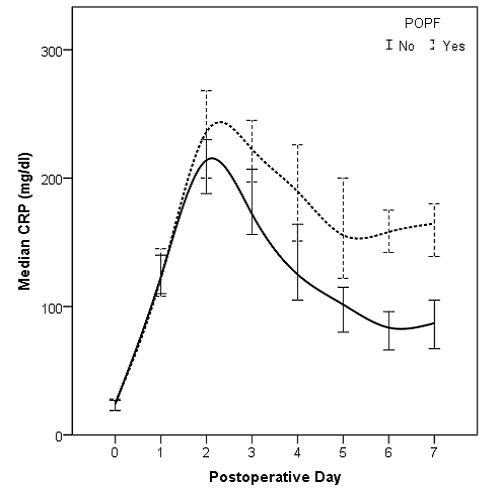
\includegraphics[width=\textwidth]{Figures/crp_comp_crp_popf_yes_no}
		\caption{POPF Absent vs. Any Grade}
		\label{fig:crp_comp_crp_popf_yes_no}
	\end{subfigure}
	\hfill
	\begin{subfigure}{0.48\textwidth}
		\centering
		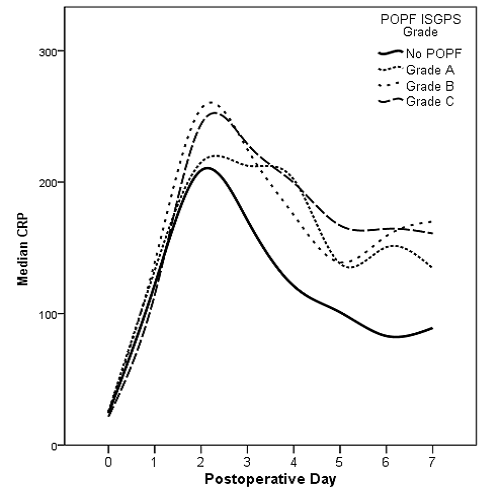
\includegraphics[width=\textwidth]{Figures/crp_comp_crp_popf_isgps}
		\caption{POPF ISGPF Grades}
		\label{fig:crp_comp_crp_popf_isgps}
	\end{subfigure}
\end{figure}
\hfill
%06/07/15 - Started this table
\begin{table}[h]
	\centering
	\caption{The relationship between CRP during the first postoperative week and post-operative pancreatic fistula (POPF) in patients undergoing pancreaticoduodenectomy.}
	\label{table:crp_comp_vs_POPF_ISGPS_p_values_only}
	\renewcommand{\arraystretch}{1.2} %Increases space between rows
	%\setlength{\tabcolsep}{9pt} %sets the space between columns
	\begin{tabular}{| c | c c c c |}
		\hline
		           &       \multicolumn{4}{c|}{POPF ISGPS Grades - \textit{p}}        \\
		Postop Day & No vs. Any Grade & No vs. A & A vs. B & B vs. C                 \\ \hline
		0          & 0.722            & 0.582    & 0.849   & 0.730                   \\
		1          & 0.242            & 0.331    & 0.740   & 0.295                   \\
		2          & 0.002            & 0.161    & 0.222   & 0.563                   \\
		3          & $<$0.001         & 0.022    & 0.602   & 0.530                   \\
		4          & $<$0.001         & 0.007    & 0.906   & 0.834                   \\
		5          & $<$0.001         & 0.035    & 0.611   & 0.959                   \\
		6          & $<$0.001         & 0.012    & 0.638   & 0.781                   \\
		7          & $<$0.001         & 0.006    & 0.235   & 0.356                   \\ \hline
		\multicolumn{5}{l}{\textit{p} - Mann-Whitney U test}                         \\
		\multicolumn{5}{l}{ISGPS - International Study Group for Pancreatic Surgery}	\\
				\multicolumn{5}{l}{POPF - Postoperative Pancreatic Fistula}
	\end{tabular}
	
	
\end{table}
%==============================================================================
\clearpage

\subsection{Postoperative CRP and infective complications}
The median CRP levels on or after postoperative day 3 were significantly higher in patients who developed clinically significant infective complications in the absence of a POPF (Fig. \ref{fig:crp_comp_infective_leak0}). Moreover, the median difference in CRP also increases from 56 mg/L on the third day to 79 mg/L on the seventh day. However, there was no such association in patients who did develop a POPF (Fig. \ref{fig:crp_comp_infective_leak1}).  For instance, difference in median CRP on Day 4 in patients who did not develop a POPF and did not have an infective complication was 97 mg/L (IQR 71 - 174) but was 173 mg/L if they had an infective complication. (p$<$0.001). However, in patients who had POPF, the CRP on day 4 was 214 mg/L (IQR 151 - 250) in the absence of infective complications and 190 mg/L (IQR 137 - 252) in the presence of infective complications. (p = 0.559)

Therefore, CRP on or after the third postoperative day appears to be useful in predicting infective complications only in patients who did not develop a POPF and these results are shown in Table \ref{table:crp_comp_vs_infections_popf_y1n0} and Fig. \ref{fig:crp_comp_infective_leak} on p\pageref{fig:crp_comp_infective_leak}. 

%========================CRP vs Infections====================================
%CRP trends vs infections in patients with or without popf in a 2-panel figure and table showing median, iqr and p-values below it
\clearpage
\begin{figure}[t]
	\caption{Relationship between postoperative CRP and clinically significant infective complications in patients without (A) and with (B) POPF.}
	\label{fig:crp_comp_infective_leak}
	\centering
	\begin{subfigure}{0.48\textwidth}
		\centering
		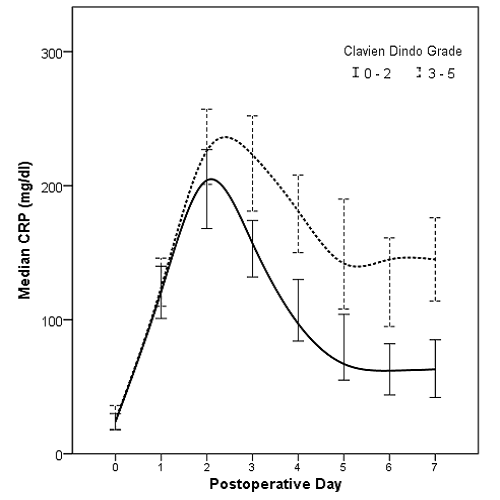
\includegraphics[width=\textwidth]{Figures/crp_comp_infective_leak0}
		\caption{Patients with \textbf{\underline{no}} POPF}
		\label{fig:crp_comp_infective_leak0}
	\end{subfigure}
	\hfill
	\begin{subfigure}{0.48\textwidth}
		\centering
		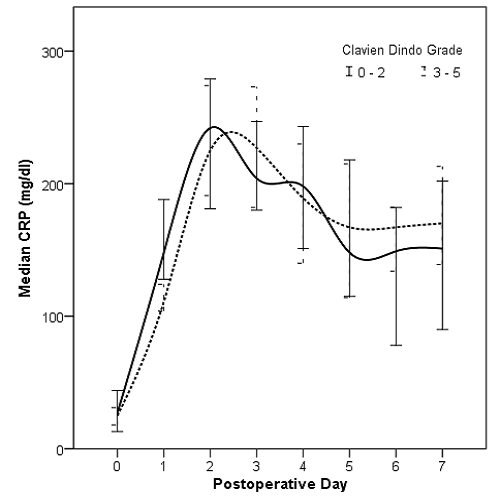
\includegraphics[width=\textwidth]{Figures/crp_comp_infective_leak1}
		\caption{Patients with POPF}
		\label{fig:crp_comp_infective_leak1}
	\end{subfigure}
\end{figure}
\vfill
%07/07/15 - Started this table
\begin{table}[h]
	\centering
	\caption{The relationship between postoperative CRP and infectious complications grouped by POPF. (Mann-Whitney U test)}
	\label{table:crp_comp_vs_infections_popf_y1n0}
	%\renewcommand{\arraystretch}{1.1} %Increases space between rows
	%\setlength{\tabcolsep}{9pt} %sets the space between columns
	\begin{tabular}{| c | c c c | c c c |}
		\hline
		           &       \multicolumn{3}{c}{POPF Absent}       &      \multicolumn{3}{c}{POPF Present}       \\
		           & \multicolumn{3}{c}{Infectious Complication} & \multicolumn{3}{c}{Infectious Complication} \\
		Postop Day & No          & Yes         & p               & No          & Yes         & p               \\
		           & (n=85)      & (n=41)      &                 & (n=19)      & (n=43)      &  \\ \hline
		0          & 24          & 25          & 0.379           & 27          & 25          & 0.629           \\
		           & (12 - 42)   & (14 - 41)   &                 & (13 - 44)   & (16 - 34)   &  \\
		1          & 122         & 123         & 0.667           & 148         & 116         & 0.038           \\
		           & (85 - 156)  & (87 - 148)  &                 & (114 - )    & (94 - 161)  &  \\
		2          & 204         & 218         & 0.203           & 242         & 228         & 0.919           \\
		           & (136 - 242) & (165 - 262) &                 & (181 - 279) & (186 - 296) &  \\
		3          & 157         & 213         & 0.011           & 206         & 226         & 0.846           \\
		           & (105 - 211) & (150 - 258) &                 & (180 - 297) & (175 - 281) &  \\
		4          & 97          & 173         & $<$0.001        & 214         & 190         & 0.559           \\
		           & (71 - 174)  & (118 - 216) &                 & (151 - 250) & (137 - 252) &  \\
		5          & 76          & 122         & $<$0.001        & 140         & 167         & 0.639           \\
		           & (40 - 129)  & (87 - 202)  &                 & (115 - 218) & (111 - 222) &  \\
		6          & 64          & 121         & $<$0.001        & 148         & 168         & 0.275           \\
		           & (31 - 133)  & (87 - 172)  &                 & (78 - 182)  & (109 - 224) &  \\
		7          & 62          & 141         & $<$0.001        & 158         & 167         & 0.644           \\
		           & (25 - 106)  & (90 - 190)  &                 & (90 - 231)  & (101 - 226) &  \\ \hline
		\multicolumn{7}{l}{Values are median (inter-quartile range.)}                                          \\
		\multicolumn{7}{l}{p - Mann-Whitney U test)}
	\end{tabular}
\end{table}
%==============================================================================
\clearpage

\subsection{Postoperative white cell counts, albumin and infective complications}

Patients who developed infective complications in the absence of POPF had a raised total white cell counts on postoperative days 5, 6 and 7 which were statistically significant However, these differences were small with wide, overlapping 95\% confidence intervals (Fig. \ref{fig:crp_comp_WCC_infective_leak0}) and not clinically significant. For instance, the median white cell count on the fifth postoperative day in patients who did not have an infective complication was 8.9 (IQR 6.6 - 11) while in patients who had an infective complication it was 9.8 (IQR 7.9 - 13). While this difference was statistically significant (p = 0.028), both medians were within the normal limits for healthy adults. There was no association between white cell counts and infective complications in patients who had a POPF. (Table \ref{table:crp_comp_WCC_vs_infections_popf_y1n0} and Fig. \ref{fig:crp_comp_WCC_infective_leak} on p\pageref{fig:crp_comp_WCC_infective_leak})

Similar statistically significant differences were noted in the postoperative neutrophil counts on postoperative days 5, 6 and 7 in patients without a POPF while there was no difference in patients with a POPF. (Table \ref{table:crp_comp_Neutrophil_vs_infections_popf_y1n0})	However, these differences were associated with a large overlap between the 95\% confidence intervals (error bars in Fig. \ref{fig:crp_comp_Neutrophil_infective_leak0}).

Patients with infective complications in the absence of POPF had a lower median serum albumin  during the entire first postoperative week with statistically significant differences from days 3 through 7. There was no association between serum albumin and infective complications in patients who had a POPF. (Table \ref{table:crp_comp_Albumin_vs_infections_popf_y1n0} and Fig. \ref{fig:crp_comp_Albumin_infective_leak} on p\pageref{fig:crp_comp_Albumin_infective_leak})

%========================WCC vs Infections====================================
%WCC trends vs infections in patients with or without popf in a 2-panel figure and table showing median, iqr and p-values below it
\clearpage
\begin{figure}[t]
	\caption{Relationship between postoperative white cell count and clinically significant infective complications in patients without (A) and with (B) POPF.}
	\label{fig:crp_comp_WCC_infective_leak}
	\centering
	\begin{subfigure}{0.48\textwidth}
		\centering
		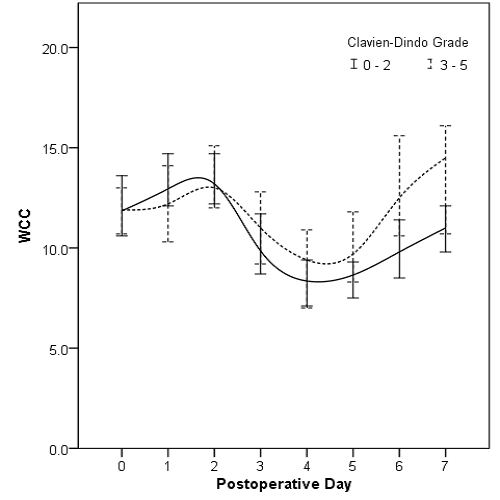
\includegraphics[width=\textwidth]{Figures/crp_comp_WCC_infective_leak0}
		\caption{Patients with \textbf{\underline{no}} POPF}
		\label{fig:crp_comp_WCC_infective_leak0}
	\end{subfigure}
	\hfill
	\begin{subfigure}{0.48\textwidth}
		\centering
		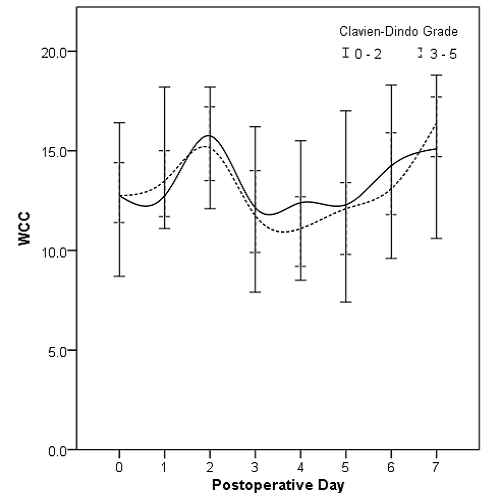
\includegraphics[width=\textwidth]{Figures/crp_comp_WCC_infective_leak1}
		\caption{Patients with POPF}
		\label{fig:crp_comp_WCC_infective_leak1}
	\end{subfigure}
\end{figure}
\vfill
%13/07/15 - Started this table
\begin{table}[h]
	\centering
	\caption{The relationship between postoperative white cell count and infective complications grouped by POPF. (Mann-Whitney U test)}
	\label{table:crp_comp_WCC_vs_infections_popf_y1n0}
	%\renewcommand{\arraystretch}{1.1} %Increases space between rows
	%\setlength{\tabcolsep}{9pt} %sets the space between columns
	\begin{tabular}{| c | c c c | c c c |}
		\hline
		           &       \multicolumn{3}{c|}{POPF Absent}       &      \multicolumn{3}{c|}{POPF Present}       \\
		           & \multicolumn{3}{c|}{Infective Complication} & \multicolumn{3}{c|}{Infective Complication} \\
		Postop Day & No            & Yes           & p            & No            & Yes           & p            \\
		           & (n=85)        & (n=41)        &              & (n=19)        & (n=43)        &  \\ \hline
		0          & 12.1          & 11.9          & 0.843        & 12.6          & 12.6          & 0.658        \\
		           & (9.7 - 14.6)  & (9.8 - 15.6)  &              & (8 - 16.4)    & (10.1 - 15.4) &  \\
		1          & 13.0          & 12.7          & 0.297        & 13.6          & 13.6          & 0.708        \\
		           & (11.6 - 15.8) & (9.5 - 16.4)  &              & (11.1 - 18.2) & (10.6 - 16.4) &  \\
		2          & 13.6          & 13.7          & 0.998        & 14.5          & 14.8          & 0.754        \\
		           & (11.3 - 16.9) & (10.5 - 17.2) &              & (10.8 - 18.2) & (12.4 - 19.3) &  \\
		3          & 9.9           & 11.0          & 0.223        & 12.0          & 11.7          & 0.843        \\
		           & (8.1 - 13.3)  & (8.6 - 14.9)  &              & (7.9 - 16.2)  & (8.2 - 15.3)  &  \\
		4          & 8.4           & 9.4           & 0.095        & 12.1          & 11.1          & 0.523        \\
		           & (6.5 - 10.8)  & (6.8 - 13.4)  &              & (8.5 - 15.5)  & (8.7 - 12.9)  &  \\
		5          & 8.9           & 9.8           & 0.028        & 12.3          & 12.3          & 0.849        \\
		           & (6.6 - 11)    & (7.9 - 13)    &              & (7.4 - 17)    & (9.5 - 14.7)  &  \\
		6          & 9.8           & 12.5          & 0.007        & 14.3          & 13.6          & 0.782        \\
		           & (7.8 - 13.2)  & (9.9 - 16)    &              & (9.6 - 18.3)  & (10.8 - 16.7) &  \\
		7          & 11.2          & 14.6          & 0.003        & 14.9          & 16.4          & 0.302        \\
		           & (9 - 14.1)    & (10.5 - 18.7) &              & (10.6 - 18.8) & (14.5 - 19.4) &  \\ \hline
		\multicolumn{7}{l}{Values are median (inter-quartile range)}                                            \\
		\multicolumn{7}{l}{p - Mann-Whitney U test}
	\end{tabular}
\end{table}
%==============================================================================

%==========Neutrophil-Neutrophil-Neutrophil-Neutrophil-Neutrophil-Neutrophil=====
%Neutrophil trends vs infections in patients with or without popf in a 2-panel figure and table showing median, iqr and p-values below it
\clearpage
\begin{figure}[t]
	\caption{Relationship between postoperative neutrophil count and clinically significant infective complications in patients without (A) and with (B) POPF.}
	\label{fig:crp_comp_Neutrophil_infective_leak}
	\centering
	\begin{subfigure}{0.48\textwidth}
		\centering
		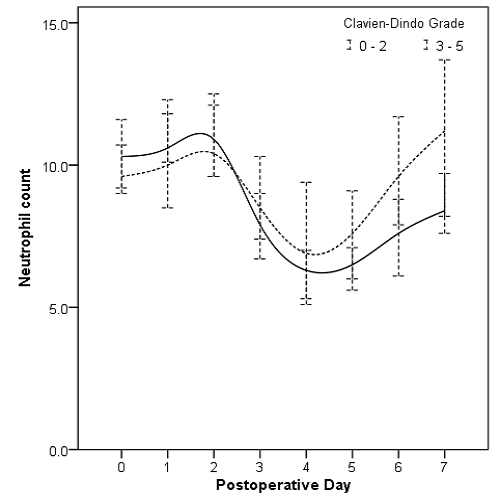
\includegraphics[width=\textwidth]{Figures/crp_comp_Neutrophil_infective_leak0}
		\caption{Patients with \textbf{\underline{no}} POPF}
		\label{fig:crp_comp_Neutrophil_infective_leak0}
	\end{subfigure}
	\hfill
	\begin{subfigure}{0.48\textwidth}
		\centering
		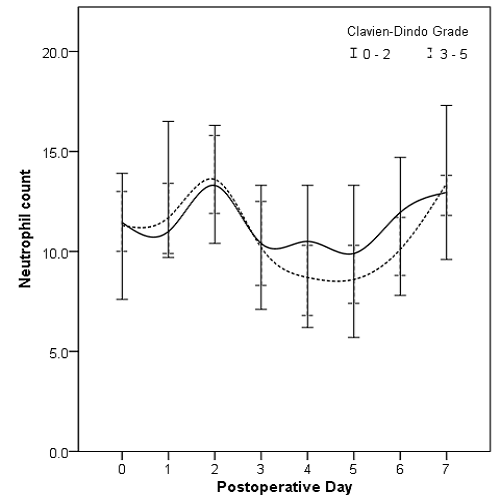
\includegraphics[width=\textwidth]{Figures/crp_comp_Neutrophil_infective_leak1}
		\caption{Patients with POPF}
		\label{fig:crp_comp_Neutrophil_infective_leak1}
	\end{subfigure}
\end{figure}
\vfill
%13/07/15 - Started this table
\begin{table}[h]
	\centering
	\caption{The relationship between postoperative neutrophil count and infectious complications grouped by POPF.}
	\label{table:crp_comp_Neutrophil_vs_infections_popf_y1n0}
	%\renewcommand{\arraystretch}{1.1} %Increases space between rows
	%\setlength{\tabcolsep}{9pt} %sets the space between columns
	\begin{tabular}{| c | c c c | c c c |}
		\hline
		           &       \multicolumn{3}{c|}{POPF Absent}       &      \multicolumn{3}{c|}{POPF Present}       \\
		           & \multicolumn{3}{c|}{Infectious Complication} & \multicolumn{3}{c|}{Infectious Complication} \\
		Postop Day & No           & Yes          & p             & No           & Yes           & p            \\
		           & (n=85)       & (n=41)       &               & (n=19)       & (n=43)        &  \\ \hline
		0          & 10.5         & 9.9          & 0.694         & 11.4         & 11.0          & 0.840 \\
		           & (8.4 - 12.7) & (8.5 - 13.9) &               & (7.3 - 13.9) & (8.6 - 13.5)  &  \\
		1          & 10.6         & 10.4         & 0.517         & 11.3         & 11.6          & 0.375 \\
		           & (9.1 - 13.2) & (7.7 - 14.2) &               & (9.7 - 16.5) & (8.5 - 13.8)  &  \\
		2          & 10.9         & 11.3         & 0.704         & 12.8         & 12.1          & 0.843 \\
		           & (8.7 - 13.9) & (9.4 - 14.2) &               & (8.6 - 16.3) & (10.5 - 16.5) &  \\
		3          & 7.9          & 8.5          & 0.086         & 10.1         & 10.1          & 0.855 \\
		           & (6 - 10.9)   & (7.1 - 12.2) &               & (7.1 - 13.3) & (7 - 13.3)    &  \\
		4          & 6.3          & 7.0          & 0.072         & 10.2         & 9.0           & 0.445 \\
		           & (4.8 - 8.4)  & (5.2 - 10.8) &               & (6.2 - 13.3) & (6.5 - 10.8)  &  \\
		5          & 6.6          & 7.6          & 0.021         & 9.9          & 9.1           & 0.693 \\
		           & (4.7 - 8.3)  & (5.6 - 10.7) &               & (5.7 - 13.3) & (7.1 - 11.3)  &  \\
		6          & 7.6          & 9.6          & 0.004         & 12.0         & 10.5          & 0.675 \\
		           & (5.8 - 9.7)  & (7.5 - 13.1) &               & (7.8 - 14.7) & (8 - 13.1)    &  \\
		7          & 8.7          & 11.6         & 0.001         & 12.4         & 13.4          & 0.412 \\
		           & (6.7 - 10.8) & (7.9 - 16.1) &               & (8.6 - 17.3) & (11.5 - 15.9) &  \\ \hline
		\multicolumn{7}{l}{Values are median (inter-quartile range)}                                          \\
		\multicolumn{7}{l}{p - Mann-Whitney U test}
	\end{tabular}
\end{table}

%==============================================================================

%==========Albumin-Albumin-Albumin-Albumin-Albumin-Albumin-Albumin-Albumin-=====
%Albumin trends vs infections in patients with or without popf in a 2-panel figure and table showing median, iqr and p-values below it
\clearpage
\begin{figure}[t]
	\caption{Relationship between postoperative serum albumin and clinically significant infective complications in patients without (A) and with (B) POPF.}
	\label{fig:crp_comp_Albumin_infective_leak}
	\centering
	\begin{subfigure}{0.48\textwidth}
		\centering
		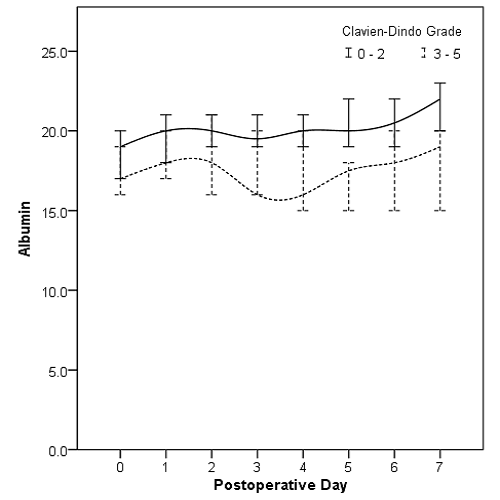
\includegraphics[width=\textwidth]{Figures/crp_comp_Albumin_infective_leak0}
		\caption{Patients with \textbf{\underline{no}} POPF}
		\label{fig:crp_comp_Albumin_infective_leak0}
	\end{subfigure}
	\hfill
	\begin{subfigure}{0.48\textwidth}
		\centering
		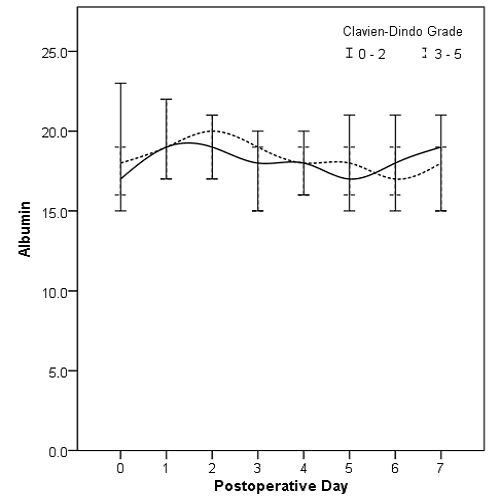
\includegraphics[width=\textwidth]{Figures/crp_comp_Albumin_infective_leak1}
		\caption{Patients with POPF}
		\label{fig:crp_comp_Albumin_infective_leak1}
	\end{subfigure}
\end{figure}
\vfill
%13/07/15 - Started this table
\begin{table}[b]
	\centering
	\caption{The relationship between postoperative serum albumin and infective complications grouped by POPF. (Mann-Whitney U test)}
	\label{table:crp_comp_Albumin_vs_infections_popf_y1n0}
	%\renewcommand{\arraystretch}{1.1} %Increases space between rows
	%\setlength{\tabcolsep}{9pt} %sets the space between columns
	\begin{tabular}{| c | c c c | c c c |}
		\hline
		           &       \multicolumn{3}{c|}{POPF Absent}       &      \multicolumn{3}{c|}{POPF Present}       \\
		           & \multicolumn{3}{c|}{Infective Complication} & \multicolumn{3}{c|}{Infective Complication} \\
		Postop Day & No        & Yes         & p                  & No        & Yes       & p                    \\
		           & (n=85)    & (n=41)      &                    & (n=19)    & (n=43)    &  \\ \hline
		0          & 20        & 17          & 0.101              & 18        & 18        & 0.981                \\
		           & (15 - 22) & (14 - 21)   &                    & (15 - 22) & (15 - 20) &  \\
		1          & 20        & 18          & 0.115              & 20        & 19        & 0.612                \\
		           & (16 - 23) & (15 - 21)   &                    & (17 - 22) & (16 - 23) &  \\
		2          & 20        & 18          & 0.090              & 18        & 19        & 0.545                \\
		           & (17 - 23) & (15 - 21.5) &                    & (15 - 21) & (16 - 22) &  \\
		3          & 20        & 16          & 0.001              & 18        & 19        & 0.689                \\
		           & (17 - 22) & (13 - 20)   &                    & (15 - 20) & (15 - 20) &  \\
		4          & 20        & 16          & $<$0.001           & 17        & 18        & 0.945                \\
		           & (17 - 23) & (14 - 20)   &                    & (16 - 19) & (15 - 20) &  \\
		5          & 20        & 18          & $<$0.001           & 16        & 18        & 0.667                \\
		           & (17 - 23) & (13.5 - 20) &                    & (15 - 20) & (15 - 20) &  \\
		6          & 20        & 18          & 0.001              & 17        & 17        & 0.981                \\
		           & (18 - 24) & (14 - 20)   &                    & (15 - 20) & (15 - 20) &  \\
		7          & 22        & 19          & $<$0.001           & 18        & 18        & 0.655                \\
		           & (18 - 25) & (14 - 20)   &                    & (15 - 20) & (15 - 21) &  \\ \hline
		\multicolumn{7}{l}{Values are median (inter-quartile range)}                                             \\
		\multicolumn{7}{l}{p - Mann-Whitney U test}
	\end{tabular}
\end{table}

%=============================================================================
\clearpage

\subsection{Receiver operating characteristic (ROC) analysis}
Receiver operating characteristic (ROC) analysis was undertaken in order to find the optimum threshold for the relationship between CRP and infective complications in patients without POPF. ROC curves were plotted with CR as a continuous variable and infective complications as a dichotomous outcome variable for postoperative days 3 through 7. 

The area under curve (AUC) was significantly higher than 0.5 for CRP on days 3 though 7. The optimum thresholds along with the corresponding sensitivity, specificity, negative predictive value, positive predictive value, 95\% confidence intervals (CI) and p-values are shown in Table \ref{table:crp_comp_ROC_infections_noPOPF} and the corresponding ROC curves are shown in Fig. \ref{fig:crp_comp_ROC_infection} on p\pageref{fig:crp_comp_ROC_infection}. The thresholds were identified with a bias towards a higher negative predictive value to allow identification of patients who did not develop an infective complication. A CRP level of 125 mg/L on the fourth postoperative day had a sensitivity of 74\% and specificity of 64\% with a negative predictive value of 83\% for predicting infective complications (AUC 0.71, 95\%CI 0.61 - 0.80, p$<$0.001). The AUC improved to 0.80 on day 7 but only with a modest increase in the negative predictive value to 87\%, with corresponding sensitivity, specificity of 65\% and 81\% respectively (95\%CI 0.72 - 0.88, p$<$0.001).

The relationship between CRP on the fourth day and other postoperative events is shown in Table \ref{table:crp_comp_CRP4_vs_LOS}. There were no deaths in this group of patients who did not have a POPF. 

%SPSS results and graphs are stored in crp_complications_graphs_etc.spv file

%========================ROC Curves==========================================
\clearpage
\begin{figure}[t]
	\caption{Receiver operating characteristics curve analysis of C-reactive protein as a marker of postoperative infective complications.}
	\label{fig:crp_comp_ROC_infection}

	\centering
	\begin{subfigure}{0.3\textwidth}
		\centering
		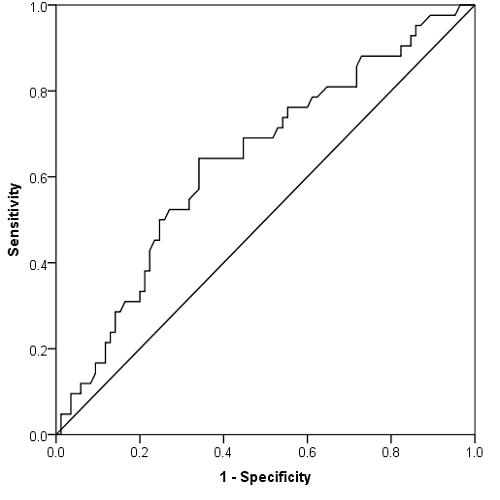
\includegraphics[width=\textwidth]{Figures/crp_comp_ROC_infection_D3}
		\caption{Day 3}
		\label{fig:crp_comp_ROC_infection_D3}
	\end{subfigure}
	\hfill
	\begin{subfigure}{0.3\textwidth}
		\centering
		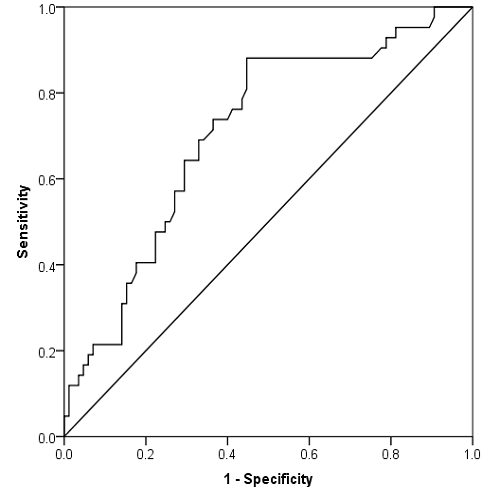
\includegraphics[width=\textwidth]{Figures/crp_comp_ROC_infection_D4}
		\caption{Day 4}
		\label{fig:crp_comp_ROC_infection_D4}
	\end{subfigure}
	\hfill
	\begin{subfigure}{0.3\textwidth}
		\centering
		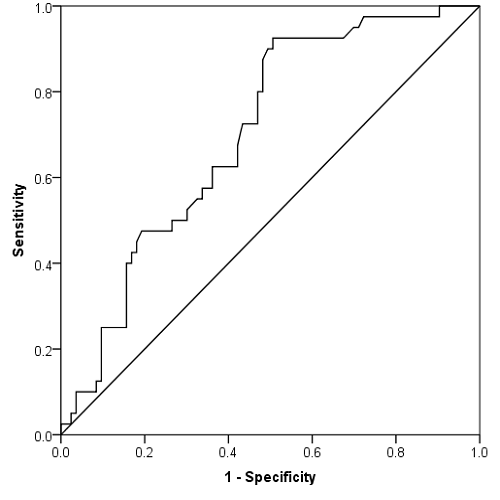
\includegraphics[width=\textwidth]{Figures/crp_comp_ROC_infection_D5}
		\caption{Day 5}
		\label{fig:crp_comp_ROC_infection_D5}
	\end{subfigure}
	\begin{subfigure}{0.3\textwidth}
		\centering
		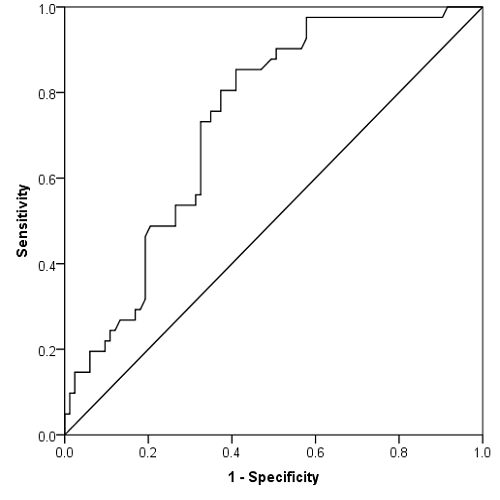
\includegraphics[width=\textwidth]{Figures/crp_comp_ROC_infection_D6}
		\caption{Day 6}		
		\label{fig:crp_comp_ROC_infection_D6}
	\end{subfigure}
	\begin{subfigure}{0.3\textwidth}
		\centering
		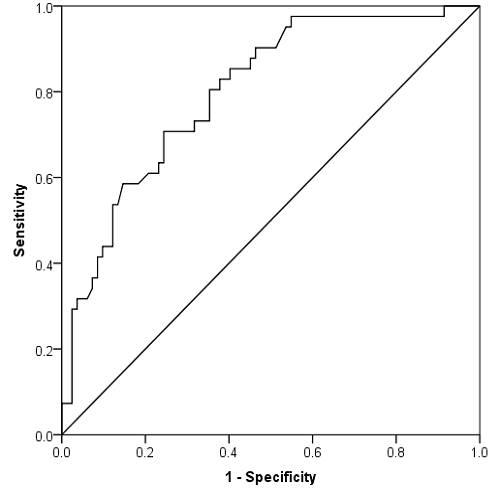
\includegraphics[width=\textwidth]{Figures/crp_comp_ROC_infection_D7}
		\caption{Day 7}
		\label{fig:crp_comp_ROC_infection_D7}
	\end{subfigure}
\end{figure}
\vfill
%07/07/15 - Started this table
\begin{table}[h]
	\centering
	\caption{Receiver operating characteristics curve analysis of C-reactive protein as a marker of postoperative infective complications in patients who did not develop a POPF}
	\label{table:crp_comp_ROC_infections_noPOPF}
	\renewcommand{\arraystretch}{1.4} %Increases space between rows
	%\setlength{\tabcolsep}{9pt} %sets the space between columns
	\begin{tabular}{| c | c c c | c c c c c |}
		\hline
		Day & AUC  & p        & 95\% CI     & CRP & Spec. & Sens. & NPV  & PPV               \\ \hline
		3   & 0.64 & 0.011    & 0.54 - 0.74 & 178 & 0.66  & 0.64  & 0.79 & 0.48              \\
		4   & 0.71 & $<$0.001 & 0.61 - 0.80 & 125 & 0.64  & 0.74  & 0.83 & 0.50              \\
		5   & 0.70 & $<$0.001 & 0.61 - 0.80 & 107 & 0.64  & 0.63  & 0.78 & 0.45              \\
		6   & 0.73 & $<$0.001 & 0.65 - 0.82 & 92  & 0.68  & 0.73  & 0.84 & 0.53              \\
		7   & 0.80 & $<$0.001 & 0.72 - 0.88 & 87  & 0.65  & 0.81  & 0.87 & 0.52              \\ \hline
		\multicolumn{9}{l}{AUC - Area under curve, Spec. - Specificity, Sens. - Sensitivity} \\
		\multicolumn{9}{l}{NPV - Negative Predictive Value, PPV - Positive Predictive Value}
	\end{tabular}
\end{table}
%=============================================================================

%===================CRP Day 4 vs LOS=========================================

%12/07/15 - Started this table
\begin{table}[p]
	\centering
	\caption{The relationship between CRP on Day 4 and other postoperative events in patients with no POPF.}
	\label{table:crp_comp_CRP4_vs_LOS}
	\renewcommand{\arraystretch}{1.4} %Increases space between rows
	\setlength{\tabcolsep}{9pt} %sets the space between columns
	\begin{tabular}{|l l  c c r |}
		\hline
		                      &          & \multicolumn{2}{c}{Day 4 CRP (mg/l)} &  \\
		                      &          & $\leq$125   & $>$125                   & \textit{p}   \\ \hline
		Postoperative stay    & Days     & 12 (9 - 16) & 15 (13 - 26)             & $<$0.001$^a$ \\
		(days)                & $\leq$14 & 43 (66.2\%) & 30 (49.2\%)              & $<$0.054$^b$ \\
		                      & $>$14    & 22 (33.8\%) & 31 (50.8\%)              &  \\
		Critical care stay    & Days     & 6 (4 - 7)   & 7 (5 - 10)               & 0.001$^a$    \\
		(days)                & $\leq$7  & 57 (87.7\%) & 38 (62.3\%)              & 0.001$^b$    \\
		                      & $>$7     & 8 (12.3\%)  & 23 (37.7\%)              &  \\
		Crit. care admissions & 1        & 60 (92.3\%) & 48 (78.7\%)              & 0.029$^b$    \\
		                      & $>$1     & 5 (7.7\%)   & 13 (21.3\%)              &  \\
		Reoperation           & No       & 63 (96.9\%) & 57 (93.4\%)              & $<$0.359$^b$ \\
		                      & Yes      & 2 (3.1\%)   & 4 (6.6\%)                &  \\ \hline
		\multicolumn{5}{l}{a - Mann-Whitney U test; b - Chi-square test}
	\end{tabular}
	\medskip
	\begin{flushleft}
		In patients who did not develop a postoperative pancreatic fistula (n=126), CRP $\leq$ 125 mg/l on the fourth postoperative day was associated with shorter stay in hospital, fewer days in critical care and lower rate of readmission to critical care.
	\end{flushleft}
\end{table}





%Quick analysis of CPET vs postop CRP - maybe one table
%ROC analysis of CRP vs LOS
%Multivariate analysis of CRP as continuous or categorical vs complications, 
\clearpage
\section{Discussion}

The results of the present study show that the severity of the postoperative systemic inflammatory response as measured by serial serum CRP levels in the first week is associated with postoperative complications after pancreaticoduodenectomy. While numerous studies have reported on a variety of methods to predict as well as diagnose POPF, few have reported on the role of CRP in predicting complications other than POPF.

The introduction of the ISGPF definition for POPF has made the diagnosis of this complication simple and uniform. The rate of POPF before the standardised definition was introduced varied anywhere between 2\% and 40\%. However, in the post-ISGPF era, the rate of POPF in published literature has remained approximately 25\%. The sole criterion for the diagnosis of POPF is a drain amylase content on or after the third postoperative day three times the upper limit of normal for serum amylase in the testing laboratory. 

In the present study, while CRP was significantly greater in patients with POPF, this difference did not occur until the second postoperative day and therefore had no further clinical use in the prediction of this complication. The early rise in CRP in patients who developed a POPF is expected as the most common risk factors for POPF are encountered intra-operatively including soft pancreatic texture, small pancreatic duct size and operative blood loss. Soft pancreatic texture has in fact been reported to be associated with elevated CRP levels after pancreaticoduodenectomy.\parencite{murakami_soft_2008}

However, the magnitude of increase in CRP during the first postoperative week was not associated with the severity of POPF. This lack of association appears to suggest that the determinants of the severity of POPF may occur later in the postoperative course and are not related to the magnitude of the initial systemic inflammatory response.

The presumed cascade of events following a POPF involves accumulation of amylase rich fluid in the peritoneal cavity around recently dissected tissues and ligated blood vessels. This can lead to localised collections that can become secondarily infected, result in erosion of blood vessels resulting in post-pancreatectomy haemorrhage, result in delayed gastric emptying or postoperative ileus as well as respiratory complications including sympathetic pleural effusions or pneumonic consolidation. In fact, most large series report a close association between POPF and PPH with the latter often following the former. The eventual outcome in patients with POPF is often determined by the cascade of complications associated with the POPF itself. In fact, all deaths in this study were in patients who developed POPF.

However, in patients without a POPF, CRP in the first week after surgery was associated with infective complications and preceded the clinical manifestation of complications. The postoperative course of patients who do not develop a POPF is not dissimilar to that in patients undergoing other major gastrointestinal resectional surgery such as colorectal or oesophago-gastric surgery. The impact of the systemic inflammatory response and the compensatory anti-inflammatory response in these patients is not confounded by the presence of POPF. Our results show that once the absence of POPF is confirmed by normal drain amylase content on the third postoperative day, serum CRP on the next (fourth) postoperative day less than 125 mg/L had a negative predictive value of 83\% in excluding an infective complication. 

The results of this study are similar to the findings of Welsch and co-workers who analysed 688 patients undergoing a variety of pancreatic resections with pancreaticojejunal anastomosis.\parencite{welsch_persisting_2008} They compared 91 patients who developed an 'inflammatory postoperative complication' with a random subset of 60 consecutive pancreatic resections. They reported that a threshold of 140 mg/L serum CRP level on the fourth postoperative day had the best diagnostic accuracy for the prediction of inflammatory postoperative complications (sensitivity 69.5\%, specificity 87.1\%, positive predictive value 48.7\% for an estimated prevalence of 15\%). However, the definitions used for POPF in this study were different from the ISGPF definition and the authors did not report on the predictive ability of CRP in the presence or absence of a POPF. Moreover, Grade A and B POPF were not included in the analysis. Our results clearly demonstrate that early CRP elevation occurs in all grades of POPF with no difference between the different grades.

In the present study, preoperative systemic inflammation as measured by the modified Glasgow Prognostic Score was not associated with infective complications. A preoperative acute phase response has been reported to be associated with an exaggerated postoperative systemic inflammatory response and septic complications. \parencite{haupt_association_1997} The modified Glasgow Prognostic Score, a validated measure of preoperative systemic inflammation, has also been reported to be associated with postoperative infective complications in patients undergoing curative colorectal resections.\parencite{moyes_preoperative_2009} The lack of association between the modified Glasgow Prognostic Score and complications in the present study may have been due to the multiple factors that are responsible for preoperative systemic inflammation in these patients including obstructive jaundice, cholangitis, biliary drainage procedures and pancreatitis consequent to intervention or pancreatic duct obstruction by tumours. These findings are similar to those reported by Dutta and co-workers who did not find any relationship between preoperative systemic inflammation and postoperative complications in patients undergoing oesophago-gastric surgery.\parencite{dutta_persistent_2011}

The difference in white cell count and neutrophil count was not clinically significant between patients who did or did not have an infective complication. This finding is similar to one of the earliest reports on the role serial CRP measurements in predicting septic complications after surgery.\parencite{mustard_c-reactive_1987} as well as in several subsequent reports. \parencite{matthiessen_increase_2008, welsch_persisting_2008, dutta_persistent_2011} The temporal association between CRP and infective complications may reflect the sensitivity of CRP as a marker of systemic inflammation. This study was not designed to look at inflammatory markers later in the postoperative period. However, Mustard and co-workers monitored CRP, white cell count and temperature for 14 days after surgery and found that CRP was the only reliable marker of septic complications.

Several mechanisms have been postulated to explain the association between postoperative CRP and complications. The most common explanation is that the CRP rise is consequent to tissue ischaemia, necrosis at the anastomotic site, bacterial translocation from the gut or bacterial infection of wounds. However, our findings and that of other authors show that the difference in CRP occurs very early in the postoperative period before infective complications become clinically manifest. 

More recently, the compensatory anti-inflammatory response with the associated immunosuppressive effects has been recognised as a possible factor in predisposing the patient to infective complications and delayed wound healing. Such an anti-inflammatory response is proportional to the initial systemic inflammatory response and therefore patients with an exaggerated inflammatory response in the immediate aftermath of surgery may be at increased risk of developing complications. Mokart and co-workers studied trends in inflammatory cytokine levels in the serum of 30 patients undergoing major abdominal surgery for cancer. They reported that the levels of anti-inflammatory cytokines IL-10 and IL-1ra were significantly greater in patients who developed infective complications and were correlated with IL-6 levels on the first postoperative day. T-cell function is also depressed after surgical trauma and the degree of suppression is related to the initial pro-inflammatory response and IL-6.\parencite{faist_immunosuppression_1997} The complex interactions between the pro and anti-inflammatory processes, neurohormonal factors of the stress response, the role of the blood-gut barrier in bacterial translocation, local factors including tissue ischaemia and damage, the immunological effects of anaesthesia, blood transfusion and hypothermia remain the subject of ongoing research.\parencite{buttenschoen_effect_2010}

%=========Strengths and limitations==========================
One of the most important strengths of this study is the separate analysis of infective complications in patients who did not develop a POPF. Other strengths of this study include the homogeneous cohort of patients all of who underwent a pancreaticoduodenectomy, the serial measurements of CRP on every day of the first postoperative week, prospective record of complications and use of the ISGPF definition for POPF. We did not measure levels of other inflammatory cytokines routinely in these patients. Future work should be aimed at characterising the inflammatory cytokine profile after pancreaticoduodenectomy to identify potential targets for immunomodulation in the perioperative period. 

In summary, the advent of enhanced recovery protocols in surgery including pancreatic surgery requires the early identification of patients not only at increased risk of complications but also those who are likely to have an uncomplicated course. This allows early identification of patients who are expected to continue on the enhanced recovery pathway and allocation of resources to improve the management of patients who are likely to develop complications. This study shows that CRP on the third postoperative day is associated with infective complications in patients undergoing pancreaticoduodenectomy who do not develop a POPF but not in patients with a POPF.
